\chapter{Mutaciones y diversificación de los genomas}\label{ch:b2:genome-diversification}

Si se siembran mil millones de bacterias en una placa con antibiótico, a
la mañana siguiente han crecido unas pocas colonias. ¿Enseñó el fármaco a
esas células a resistirlo, o eran ya resistentes antes de encontrarlo? La
pregunta suena filosófica y quedó zanjada en 1943 con un experimento de
gran elegancia: las células resistentes estaban ahí de antemano,
producidas por \omterm{def:b2:genome-diversification:mutation}{mutaciones} ocurridas al azar, sin relación con su
utilidad. Este capítulo trata de las fuentes de esa variación --- los
errores de copia, los accidentes químicos, los genes saltarines, los genes
intercambiados entre células, las duplicaciones de genes y de genomas
enteros --- y de la velocidad a la que operan. La selección, que criba la
variación, es el tema del \cref{ch:b2:population-genetics}; aquí el tema
es de dónde procede la materia prima.

\section{Las mutaciones}

\begin{definition}[La mutación y sus tipos]\label{def:b2:genome-diversification:mutation}
\index{mutación}\index{mutación puntual}\index{desplazamiento del marco de lectura}\index{reordenación cromosómica}
Una \emph{mutación} es un cambio heredable en la secuencia del genoma.
Las \emph{mutaciones puntuales} cambian una o unas pocas bases: una
\emph{sustitución} reemplaza una base por otra (una \emph{transición}
cambia una purina por otra purina o una pirimidina por otra pirimidina,
A$\leftrightarrow$G o C$\leftrightarrow$T; una \emph{transversión}
intercambia las clases); una \emph{inserción} o una \emph{deleción}
añade o elimina bases. En una secuencia codificante, una sustitución es
\emph{silenciosa} si el nuevo codón especifica el mismo aminoácido,
\emph{de sentido erróneo} si especifica otro, y \emph{sin sentido} si
crea un codón de terminación; una inserción o deleción que no es múltiplo
de tres desplaza el marco de lectura (\emph{desplazamiento del marco}) y
altera todos los codones situados aguas abajo. Las
\emph{reordenaciones cromosómicas} desplazan segmentos grandes: deleción,
duplicación, inversión, translocación entre cromosomas. Las
\emph{mutaciones genómicas} cambian el número de cromosomas:
\emph{aneuploidía} (un cromosoma de más o de menos, como en la trisomía
21) y \emph{\omterm{def:b2:genome-diversification:polyploidy}{poliploidía}} (juegos completos adicionales). Una mutación en
una célula somática solo la heredan los descendientes de esa célula; una
mutación en la línea germinal la heredan los descendientes del
organismo, y solo estas cuentan para la evolución.
\end{definition}

\begin{omfigure}
\begin{tikzpicture}[every node/.style={font=\small\ttfamily}]
  \node[anchor=west] at (0,2.4) {ATG GAA TTC CTG AAG TGG TAA};
  \node[anchor=west, font=\scriptsize\rmfamily] at (5.6,2.4) {Met Glu Phe Leu Lys Trp stop --- tipo silvestre};
  \node[anchor=west] at (0,1.7) {ATG GA\textcolor{omThm}{G} TTC CTG AAG TGG TAA};
  \node[anchor=west, font=\scriptsize\rmfamily] at (5.6,1.7) {Met Glu Phe Leu Lys Trp stop --- silenciosa};
  \node[anchor=west] at (0,1.0) {ATG G\textcolor{omThm}{T}A TTC CTG AAG TGG TAA};
  \node[anchor=west, font=\scriptsize\rmfamily] at (5.6,1.0) {Met \textcolor{omThm}{Val} Phe Leu Lys Trp stop --- de sentido erróneo};
  \node[anchor=west] at (0,0.3) {ATG \textcolor{omThm}{T}AA TTC CTG AAG TGG TAA};
  \node[anchor=west, font=\scriptsize\rmfamily] at (5.6,0.3) {Met \textcolor{omThm}{stop} --- sin sentido};
  \node[anchor=west] at (0,-0.4) {ATG GA\textcolor{omThm}{C}A TTC CTG AAG TGG TAA};
  \node[anchor=west, font=\scriptsize\rmfamily] at (5.6,-0.4) {Met \textcolor{omThm}{Asp Ile Pro Glu Val} \dots{} --- desplazamiento del marco};
\end{tikzpicture}

{\small \omterm{def:b2:genome-diversification:mutation}{Mutaciones} puntuales en una secuencia codificante corta (el
cambio, en rojo). Una sustitución silenciosa conserva la proteína; una de
sentido erróneo cambia un residuo; una sin sentido la trunca; una sola
base insertada desplaza el marco y reescribe todo lo que queda aguas
abajo.}
\end{omfigure}

\begin{proposition}[De dónde vienen las mutaciones]\label{prop:b2:genome-diversification:sources}
\index{mutágeno}\index{desaminación}\index{despurinación}
Tres fuentes. \emph{Errores de replicación}: la ADN polimerasa coloca mal
una base aproximadamente una vez de cada $10^{5}$; su exonucleasa
correctora elimina la mayoría y deja una de cada $10^{7}$; la reparación
de desapareamientos, que sigue a la horquilla de replicación y corrige la
hebra nueva frente a la antigua, lleva la tasa final de error a unos
$10^{-9}$ a $10^{-10}$ por base y por
replicación. \emph{Química espontánea}: cada día, en cada célula humana,
unas \num{10000} purinas se desprenden de su azúcar
(\emph{despurinación}) y un centenar de citosinas pierden un grupo amino
(\emph{desaminación}, que convierte C en U, que se aparea con A); ambas
lesiones se reparan, pero no siempre. \emph{Mutágenos}: la luz
ultravioleta suelda timinas adyacentes en dímeros; la radiación ionizante
rompe las hebras; los agentes alquilantes y el ácido nitroso alteran las
bases; los colorantes intercalantes se deslizan entre pares de bases y
provocan desplazamientos del marco; los radicales de oxígeno de la
respiración oxidan la guanina. La tasa por base es ínfima; multiplicada
por el tamaño de un genoma y por el número de células, no lo es.
\end{proposition}

\begin{theorem}[Mutaciones por genoma y por población]\label{thm:b2:genome-diversification:rate}
\index{tasa de mutación}
Si la \omterm{thm:b2:genome-diversification:rate}{tasa de mutación} es $u$ por par de bases y por replicación y el
genoma contiene $G$ pares de bases, cada replicación produce en promedio
$U = uG$ \omterm{def:b2:genome-diversification:mutation}{mutaciones} nuevas, y una población de $N$ células produce $UN$
por generación. Para \emph{E.~coli} ($u \approx \qty{5e-10}{}$, $G =
\qty{4.6e6}{}$): $U \approx 0.002$, de modo que una célula de cada
quinientas lleva una \omterm{def:b2:genome-diversification:mutation}{mutación} nueva --- pero un cultivo de $10^{9}$
células produce dos millones por generación, y cada uno de los $3G \approx 1.4\times
10^{7}$ cambios posibles de una sola base aparece en algún punto del
cultivo cada pocas generaciones. Para un ser humano ($u \approx \qty{1.2e-8}{}$ por
generación, $G = \qty{3.2e9}{}$ por juego haploide, dos juegos): cada
hijo lleva unas \num{75} \omterm{def:b2:genome-diversification:mutation}{mutaciones} nuevas, una o dos de ellas en
secuencia codificante.
\end{theorem}
\begin{proof}
Cada base se copia de forma independiente con una probabilidad de error
$u$, de modo que el número de errores por copia del genoma es una suma de
$G$ sucesos raros independientes, de media $uG$ (y distribuida
aproximadamente según una ley de Poisson). $N$ células hacen $N$ copias.
La cifra humana multiplica $u$ por $2G$ para el genoma diploide; la tasa
por generación es por generación y no por replicación porque las células
germinales pasan por muchas replicaciones entre una fecundación y la
siguiente.
\end{proof}

\begin{theorem}[Mutantes en un cultivo en crecimiento]\label{thm:b2:genome-diversification:luria}
\index{experimento de Luria--Delbrück}\index{test de fluctuación}
Un cultivo que crece de $N_0$ a $N$ células, en el que una \omterm{def:b2:genome-diversification:mutation}{mutación} dada
ocurre con probabilidad $m$ en cada división celular, contiene al final
un número medio de \emph{sucesos} de \omterm{def:b2:genome-diversification:mutation}{mutación} $m(N - N_0)$, y un número
medio de \emph{células} mutantes
\[
\langle M\rangle = m\,N\,\ln\frac{N}{N_0},
\]
mayor que el número de sucesos porque una \omterm{def:b2:genome-diversification:mutation}{mutación} temprana funda un
clon. El número de células mutantes varía enormemente de un cultivo a
otro (los raros sucesos tempranos dan ``premios gordos''), mientras que,
si las \omterm{def:b2:genome-diversification:mutation}{mutaciones} se indujeran al sembrar, seguiría una ley de Poisson
de varianza igual a su media. La fracción de cultivos sin ningún
mutante es $p_0 = e^{-m(N - N_0)}$, lo que da $m$ directamente.
\end{theorem}
\begin{proof}
El crecimiento de $n$ a $n + \mathrm{d}n$ células requiere $\mathrm{d}n$
divisiones, cada una ocasión para la \omterm{def:b2:genome-diversification:mutation}{mutación}, de modo que en ese
intervalo ocurren $m\,\mathrm{d}n$ sucesos; sumando, $m(N - N_0)$ sucesos
en total. Una \omterm{def:b2:genome-diversification:mutation}{mutación} que ocurre cuando el cultivo tiene $n$ células
funda un clon que crece al mismo ritmo que el cultivo y cuenta $N/n$
células al final; el número esperado de células mutantes es, por tanto,
$\int_{N_0}^{N} m\,(N/n)\,\mathrm{d}n = mN\ln(N/N_0)$. Los sucesos
son raros e independientes, así que su número sigue una ley de Poisson
de media $m(N - N_0)$, y la probabilidad de que no haya ninguno es
$e^{-m(N - N_0)}$.
\end{proof}
\begin{proof}[Evidencia]
Luria y Delbrück (1943) cultivaron veinte pequeños cultivos de
\emph{E.~coli}, cada uno a partir de unas pocas células, y en paralelo
tomaron veinte muestras de un único cultivo grande; sembraron las
cuarenta con un bacteriófago que mata a toda célula sensible y contaron
las colonias resistentes. Las muestras del cultivo único dieron recuentos
próximos a su media, como predice una ley de Poisson; los cultivos
independientes dieron recuentos de 0, 0, 1, 0, 3, 0, 107, 0, 5\dots{}
--- una varianza muchas veces superior a la media. Las \omterm{def:b2:genome-diversification:mutation}{mutaciones} a la
resistencia habían ocurrido en momentos aleatorios \emph{antes} de que
las células encontraran el fago, y las tempranas producían los premios
gordos. Lederberg y Lederberg (1952) lo confirmaron sin exponer nunca al
agente las células seleccionadas: apretando un tampón de terciopelo sobre
una placa y estampando copias, encontraron colonias resistentes en las
mismas posiciones en todas las réplicas, y las aislaron de la placa
maestra no tratada.
\end{proof}

\begin{omfigure}
\begin{tikzpicture}[every node/.style={font=\scriptsize}, level distance=0.55cm, sibling distance=0.5cm, edge from parent/.style={draw, gray}]
  \begin{scope}
    \node[circle, fill=omDef!40, inner sep=1.5pt] (r) at (0,0) {}
      child { node[circle, fill=omDef!40, inner sep=1.5pt] {}
        child { node[circle, fill=omDef!40, inner sep=1.5pt] {} child { node[circle, fill=omDef!40, inner sep=1.5pt] {} } child { node[circle, fill=omDef!40, inner sep=1.5pt] {} } }
        child { node[circle, fill=omDef!40, inner sep=1.5pt] {} child { node[circle, fill=omDef!40, inner sep=1.5pt] {} } child { node[circle, fill=omThm, inner sep=1.5pt] {} } } }
      child { node[circle, fill=omDef!40, inner sep=1.5pt] {}
        child { node[circle, fill=omDef!40, inner sep=1.5pt] {} child { node[circle, fill=omDef!40, inner sep=1.5pt] {} } child { node[circle, fill=omDef!40, inner sep=1.5pt] {} } }
        child { node[circle, fill=omDef!40, inner sep=1.5pt] {} child { node[circle, fill=omDef!40, inner sep=1.5pt] {} } child { node[circle, fill=omDef!40, inner sep=1.5pt] {} } } };
    \node[align=center] at (0,-2.4) {mutación tardía:\\una célula mutante};
  \end{scope}
  \begin{scope}[xshift=5cm]
    \node[circle, fill=omDef!40, inner sep=1.5pt] at (0,0) {}
      child { node[circle, fill=omThm, inner sep=1.5pt] {}
        child { node[circle, fill=omThm, inner sep=1.5pt] {} child { node[circle, fill=omThm, inner sep=1.5pt] {} } child { node[circle, fill=omThm, inner sep=1.5pt] {} } }
        child { node[circle, fill=omThm, inner sep=1.5pt] {} child { node[circle, fill=omThm, inner sep=1.5pt] {} } child { node[circle, fill=omThm, inner sep=1.5pt] {} } } }
      child { node[circle, fill=omDef!40, inner sep=1.5pt] {}
        child { node[circle, fill=omDef!40, inner sep=1.5pt] {} child { node[circle, fill=omDef!40, inner sep=1.5pt] {} } child { node[circle, fill=omDef!40, inner sep=1.5pt] {} } }
        child { node[circle, fill=omDef!40, inner sep=1.5pt] {} child { node[circle, fill=omDef!40, inner sep=1.5pt] {} } child { node[circle, fill=omDef!40, inner sep=1.5pt] {} } } };
    \node[align=center] at (0,-2.4) {mutación temprana:\\un premio gordo de cuatro};
  \end{scope}
  \begin{scope}[xshift=10cm]
    \node[circle, fill=omDef!40, inner sep=1.5pt] at (0,0) {}
      child { node[circle, fill=omDef!40, inner sep=1.5pt] {}
        child { node[circle, fill=omDef!40, inner sep=1.5pt] {} child { node[circle, fill=omDef!40, inner sep=1.5pt] {} } child { node[circle, fill=omThm, inner sep=1.5pt] {} } }
        child { node[circle, fill=omDef!40, inner sep=1.5pt] {} child { node[circle, fill=omDef!40, inner sep=1.5pt] {} } child { node[circle, fill=omDef!40, inner sep=1.5pt] {} } } }
      child { node[circle, fill=omDef!40, inner sep=1.5pt] {}
        child { node[circle, fill=omDef!40, inner sep=1.5pt] {} child { node[circle, fill=omThm, inner sep=1.5pt] {} } child { node[circle, fill=omDef!40, inner sep=1.5pt] {} } }
        child { node[circle, fill=omDef!40, inner sep=1.5pt] {} child { node[circle, fill=omDef!40, inner sep=1.5pt] {} } child { node[circle, fill=omDef!40, inner sep=1.5pt] {} } } };
    \node[align=center] at (0,-2.4) {inducida al sembrar:\\dispersión de Poisson};
  \end{scope}
\end{tikzpicture}

{\small El \omterm{thm:b2:genome-diversification:luria}{test de fluctuación}. Si las \omterm{def:b2:genome-diversification:mutation}{mutaciones} (rojo) ocurren al azar
durante el crecimiento, el número de mutantes depende de \emph{cuándo}
ocurrió la \omterm{def:b2:genome-diversification:mutation}{mutación}, y los cultivos independientes difieren
enormemente; si el agente selectivo las indujera al sembrar, todos los
cultivos mostrarían un número pequeño similar.}
\end{omfigure}

\begin{omfigure}
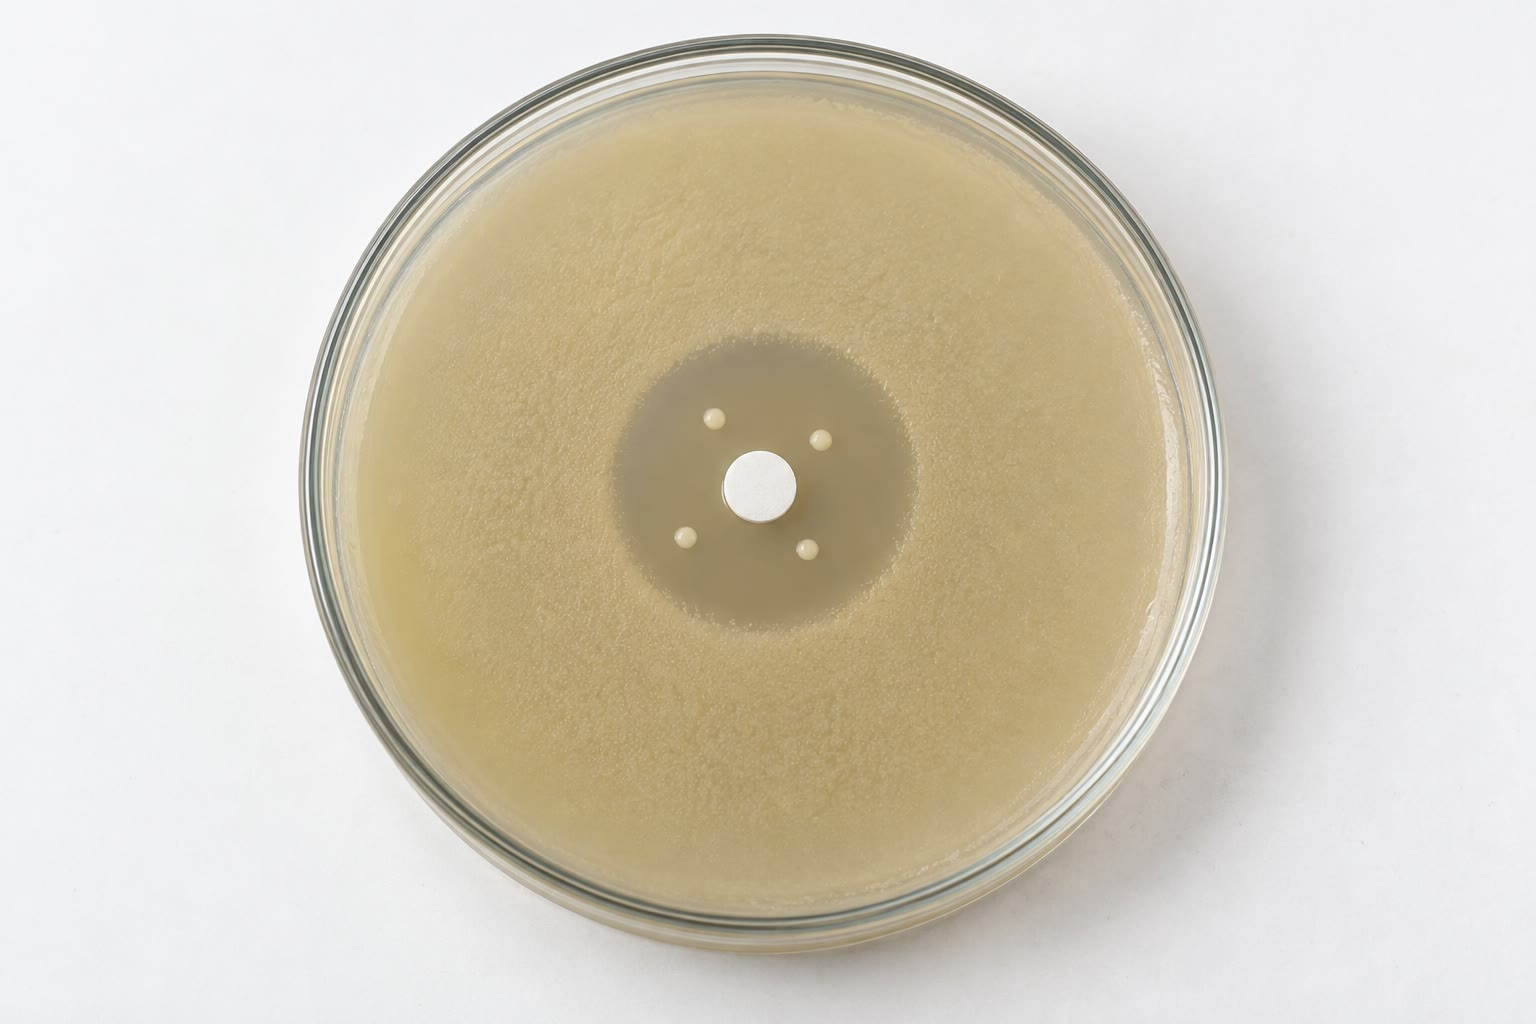
\includegraphics[width=0.5\linewidth]{images/book4/ai/b4-03-luria-plate.jpg}

{\small Un disco de antibiótico sobre un césped de bacterias: la zona
clara es donde el fármaco que difunde desde el disco ha matado a las
células sensibles, y las colonias que hay dentro crecieron a partir de
mutantes resistentes presentes antes de colocar el disco.}
\end{omfigure}

\begin{proposition}[La reparación y sus límites]\label{prop:b2:genome-diversification:repair}
\index{reparación del ADN}
Una célula corrige la mayoría de las lesiones antes de que se conviertan
en \omterm{def:b2:genome-diversification:mutation}{mutaciones}. La \emph{reparación de desapareamientos} retira la base
errónea de la hebra recién sintetizada. La \emph{reparación por escisión
de bases} recorta una sola base dañada (un uracilo, una guanina oxidada)
y rellena el hueco; por eso el ADN usa timina y no uracilo: un uracilo en
el ADN solo puede ser una citosina desaminada, y se reconoce como
extraño. La \emph{reparación por escisión de nucleótidos} retira un tramo
de una docena de bases alrededor de una lesión voluminosa, como un dímero
de timina; las personas que carecen de ella (xeroderma pigmentoso)
desarrollan cánceres de piel con la luz solar ordinaria. La
\emph{reparación por recombinación} reconstruye un cromosoma roto a partir
de su copia hermana. Lo que escapa a la reparación, o se repara mal, es
una \omterm{def:b2:genome-diversification:mutation}{mutación} --- y una célula que ha perdido un sistema de reparación (un
\emph{mutador}) muta cien veces más deprisa, lo que es una ventaja a
corto plazo bajo estrés y una carga a largo plazo. Los mecanismos de
reparación se tratan en profundidad en el volumen del tercer año.
\end{proposition}

\section{Genes que se mueven}

\begin{definition}[Elementos transponibles]\label{def:b2:genome-diversification:transposon}
\index{transposón}\index{retrotransposón}
Un \emph{elemento transponible} es un segmento de ADN capaz de desplazarse
a una nueva posición del genoma. Los \emph{transposones de ADN} codifican
una \emph{transposasa} que recorta el elemento y lo pega en otro lugar
(o lo copia allí); las secuencias de inserción bacterianas son los más
sencillos (un gen de transposasa entre dos repeticiones invertidas), y
los transposones compuestos llevan genes adicionales --- a menudo
resistencias a antibióticos --- entre dos de ellas. Los
\emph{retrotransposones} se desplazan por una vía de copiar y pegar a
través de un intermediario de ARN, que una transcriptasa inversa vuelve a
copiar en ADN; nunca abandonan su antiguo sitio y por eso se acumulan. Un
elemento que cae dentro de un gen lo interrumpe; si cae cerca, puede
alterar su expresión; dos copias en un mismo cromosoma ofrecen sitios
para un \omterm{prop:b2:genome-diversification:duplication}{entrecruzamiento desigual}. Los transposones y sus restos
constituyen la mitad del genoma humano y el ochenta por ciento del
genoma del maíz; la mayoría son hoy inmóviles.
\end{definition}
\begin{proof}[Evidencia]
McClintock (décadas de 1940 y 1950) estudió granos de maíz cuyo pigmento
púrpura se perdía en unas células y se recuperaba en otras, lo que daba
granos moteados. Mostró, mediante cruzamientos y observando los
cromosomas, que la inestabilidad se debía a un elemento
(\emph{Dissociation}) que rompía el cromosoma donde se encontraba y se
desplazaba entre posiciones bajo el control de un segundo elemento
(\emph{Activator}), y que un gen quedaba silenciado cuando el elemento se
alojaba en él y se reactivaba cuando lo abandonaba. Los genes, concluyó,
podían cambiar de posición; la idea solo se aceptó veinte años después,
cuando se descubrieron las secuencias de inserción bacterianas, y le
valió el Premio Nobel en 1983.
\end{proof}

\begin{omfigure}
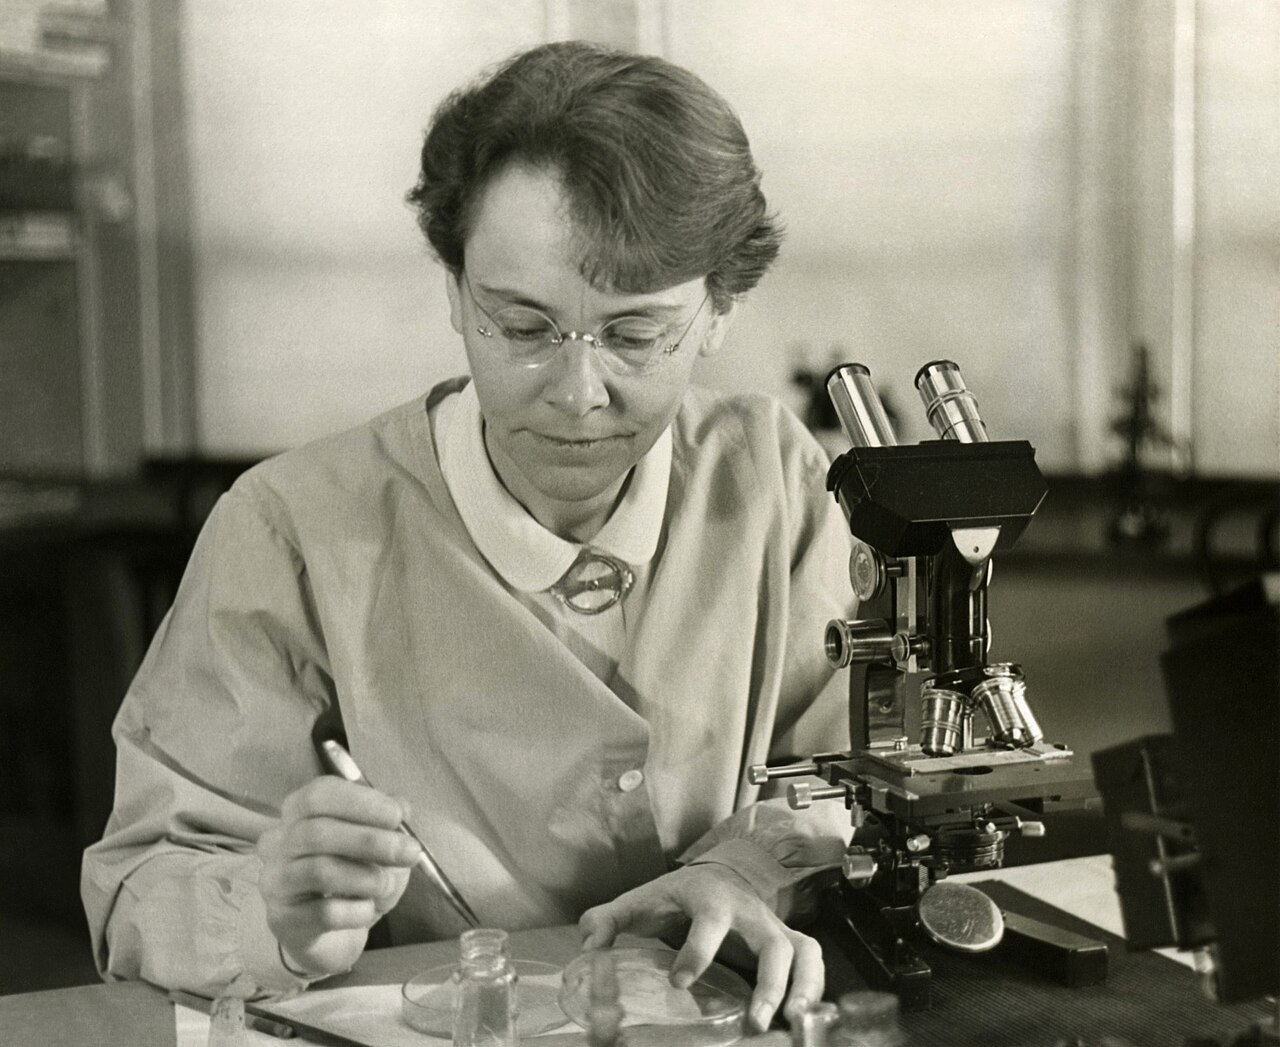
\includegraphics[width=0.4\linewidth]{images/book4/mcclintock.jpg}\hspace{0.04\linewidth}
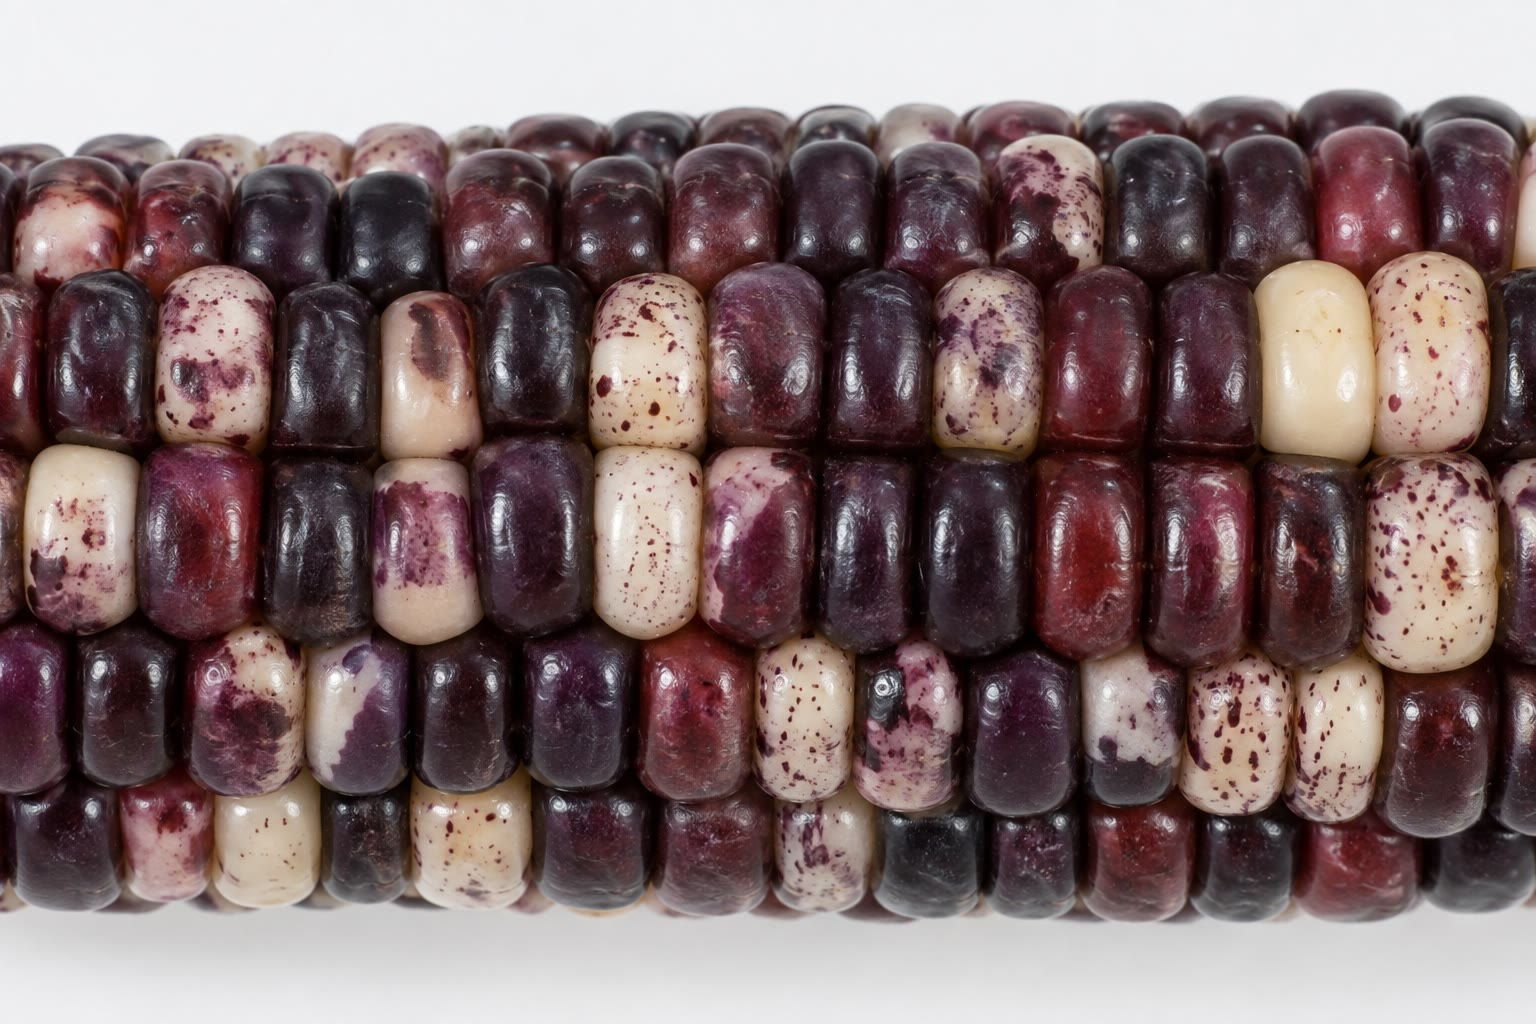
\includegraphics[width=0.5\linewidth]{images/book4/ai/b4-03-maize-kernels.jpg}

{\small Barbara McClintock y los granos que la llevaron a los elementos
transponibles: un gen del pigmento púrpura apagado por un elemento
insertado y vuelto a encender, célula a célula, cuando el elemento salta
fuera, dejando motas y sectores.}
\end{omfigure}

\begin{omfigure}
\begin{tikzpicture}[every node/.style={font=\scriptsize}]
  % cut and paste
  \begin{scope}
    \draw[very thick, gray] (0,1.2) -- (4.5,1.2);
    \fill[omThm!70] (0.8,1.05) rectangle (1.8,1.35); \node[white, font=\tiny] at (1.3,1.2) {Tn};
    \draw[very thick, gray] (0,0) -- (4.5,0);
    \fill[omThm!70] (2.8,-0.15) rectangle (3.8,0.15); \node[white, font=\tiny] at (3.3,0) {Tn};
    \draw[->, thick, omThm] (1.3,1.0) .. controls (1.3,0.5) and (3.3,0.7) .. (3.3,0.2);
    \draw[dashed, gray] (0.8,1.2) -- (1.8,1.2);
    \node[align=center] at (2.25,-0.6) {cortar y pegar (transposón de ADN):\\el elemento abandona su sitio};
  \end{scope}
  % copy and paste
  \begin{scope}[xshift=7.5cm]
    \draw[very thick, gray] (0,1.2) -- (4.5,1.2);
    \fill[omProp!80] (0.8,1.05) rectangle (1.8,1.35); \node[white, font=\tiny] at (1.3,1.2) {RT};
    \draw[very thick, gray] (0,0) -- (4.5,0);
    \fill[omProp!80] (2.8,-0.15) rectangle (3.8,0.15); \node[white, font=\tiny] at (3.3,0) {RT};
    \draw[->, thick, omProp] (1.3,1.0) .. controls (1.3,0.5) and (3.3,0.7) .. (3.3,0.2);
    \node[omProp, anchor=west, align=left] at (3.6,0.75) {copia de ARN,\\retrotranscrita};
    \node[align=center] at (2.25,-0.6) {copiar y pegar (retrotransposón):\\la copia vieja queda, el número crece};
  \end{scope}
\end{tikzpicture}

{\small Dos maneras de desplazarse. Un \omterm{def:b2:genome-diversification:transposon}{transposón} de ADN se escinde y se
reinserta; un \omterm{def:b2:genome-diversification:transposon}{retrotransposón} se transcribe, se vuelve a copiar en ADN y
se inserta en otro lugar, de modo que sus copias se acumulan.}
\end{omfigure}

\begin{definition}[Transferencia horizontal de genes]\label{def:b2:genome-diversification:hgt}
\index{transferencia horizontal de genes}\index{transformación}\index{conjugación!bacteriana}\index{transducción}
Los \omterm{def:b2:unicellular-diversity:prokaryote}{procariotas} adquieren genes de células que no son sus progenitoras
por tres vías. \emph{Transformación}: una célula capta ADN desnudo de su
entorno (liberado por células muertas) y lo recombina en su cromosoma;
algunas especies son competentes de forma natural, y es la vía por la que
los neumococos intercambian genes de la cápsula. \emph{Conjugación}: un
donante portador de un \omterm{def:b2:unicellular-diversity:prokaryote}{plásmido} conjugativo (el factor F de
\emph{E.~coli}) construye un pilus, atrae hacia sí a un receptor y le
transfiere una sola hebra del \omterm{def:b2:unicellular-diversity:prokaryote}{plásmido} a través de un poro mientras la
replica por círculo rodante; si el \omterm{def:b2:unicellular-diversity:prokaryote}{plásmido} se ha integrado en el
cromosoma (una cepa Hfr), los genes cromosómicos se transfieren en orden
tras él, y el momento en que entra cada uno cartografía el cromosoma.
\emph{Transducción}: un bacteriófago empaqueta por error un fragmento de
ADN del hospedador y lo inyecta en la siguiente célula que infecta. Entre
todas, estas vías desplazan genes de resistencia entre especies en los
hospitales en cuestión de años, y han desplazado genes metabólicos a
través de todo el árbol bacteriano a lo largo del tiempo geológico, de
modo que la ascendencia de un \omterm{def:b2:unicellular-diversity:prokaryote}{procariota} es tanto una red como un árbol
(\cref{ch:b2:phylogenetic-trees}).
\end{definition}
\begin{proof}[Evidencia]
Lederberg y Tatum (1946) mezclaron dos cepas de \emph{E.~coli}, cada una
incapaz de fabricar dos nutrientes distintos, y sembraron la mezcla en un
medio mínimo en el que ninguna podía crecer sola: aparecieron colonias,
a razón de una por cada diez millones de células, capaces de fabricar
los cuatro --- recombinantes. Davis (1950) lo repitió con las cepas
separadas por un filtro que dejaba pasar las moléculas pero no las
células: no hubo recombinantes, de modo que hacía falta contacto. Hayes
mostró después que la transferencia era unidireccional, de un donante a
un receptor, y Wollman y Jacob (1956) interrumpieron apareamientos en una
batidora a intervalos y encontraron que los genes del donante entraban
en el receptor en un orden fijo, uno tras otro, a lo largo de unos cien
minutos.
\end{proof}

\begin{omfigure}
\begin{minipage}[b]{0.56\linewidth}\centering
\begin{tikzpicture}[every node/.style={font=\scriptsize}]
  % donor
  \draw[thick, fill=omDef!8] (0,0) ellipse (1.5 and 0.75);
  \draw[thick, omDef] (0.2,0) circle (0.45);
  \draw[thick, omThm] (-0.9,0.1) circle (0.22);
  \node[anchor=south] at (0,1.25) {donante $F^+$};
  \draw[omThm] (-0.9,-0.12) -- (-1.1,-1.0) node[below] {plásmido F};
  \draw[omDef] (0.4,-0.4) -- (0.6,-1.0) node[below] {cromosoma};
  % recipient
  \draw[thick, fill=omDef!8] (5,0) ellipse (1.5 and 0.75);
  \draw[thick, omDef] (5.2,0) circle (0.45);
  \node[anchor=south] at (5,1.25) {receptor $F^-$};
  % pilus
  \draw[very thick, omThm] (1.5,0) -- (3.5,0);
  \node[omThm, below] at (2.5,-0.05) {pilus};
  % single strand transferred
  \draw[->, thick, omThm, dashed] (-0.7,0.15) .. controls (1.0,0.7) and (3.0,0.7) .. (4.1,0.4);
  \node[omThm, anchor=south] at (2.5,0.7) {una hebra copiada por círculo rodante};
  \draw[thick, omThm, dashed] (4.1,0.2) circle (0.2);
\end{tikzpicture}
\end{minipage}\hfill
\begin{minipage}[b]{0.42\linewidth}\centering
\begin{tikzpicture}
\begin{axis}[
  width=\linewidth, height=4.6cm,
  axis x line=bottom, axis y line=left,
  xmin=0, xmax=40, ymin=0, ymax=1.1,
  xlabel={minutos antes de batir}, ylabel={recombinantes (relativo)},
  xlabel style={font=\scriptsize, at={(axis description cs:0.5,-0.18)}, anchor=north},
  ylabel style={font=\scriptsize},
  tick label style={font=\scriptsize}, xtick={0,10,20,30,40}, ytick={0,0.5,1},
  legend style={font=\scriptsize, at={(0.97,0.08)}, anchor=south east, draw=none},
  clip=false,
]
\addplot[very thick, omDef, domain=8:40, samples=40] {1-exp(-(x-8)/5)};
\addlegendentry{\emph{thr}, entra a los \qty{8}{min}}
\addplot[very thick, omProp, domain=17:40, samples=40] {1-exp(-(x-17)/5)};
\addlegendentry{\emph{lac}, \qty{17}{min}}
\addplot[very thick, omThm, domain=25:40, samples=40] {1-exp(-(x-25)/5)};
\addlegendentry{\emph{gal}, \qty{25}{min}}
\end{axis}
\end{tikzpicture}
\end{minipage}

{\small Izquierda: conjugación --- el donante transfiere una hebra de su
\omterm{def:b2:unicellular-diversity:prokaryote}{plásmido} F a través de la unión del pilus mientras la copia. Derecha: el
experimento de apareamiento interrumpido con un donante Hfr: cada gen
cromosómico empieza a aparecer entre los recombinantes en un momento
característico, que cartografía el cromosoma en minutos.}
\end{omfigure}

\begin{omfigure}
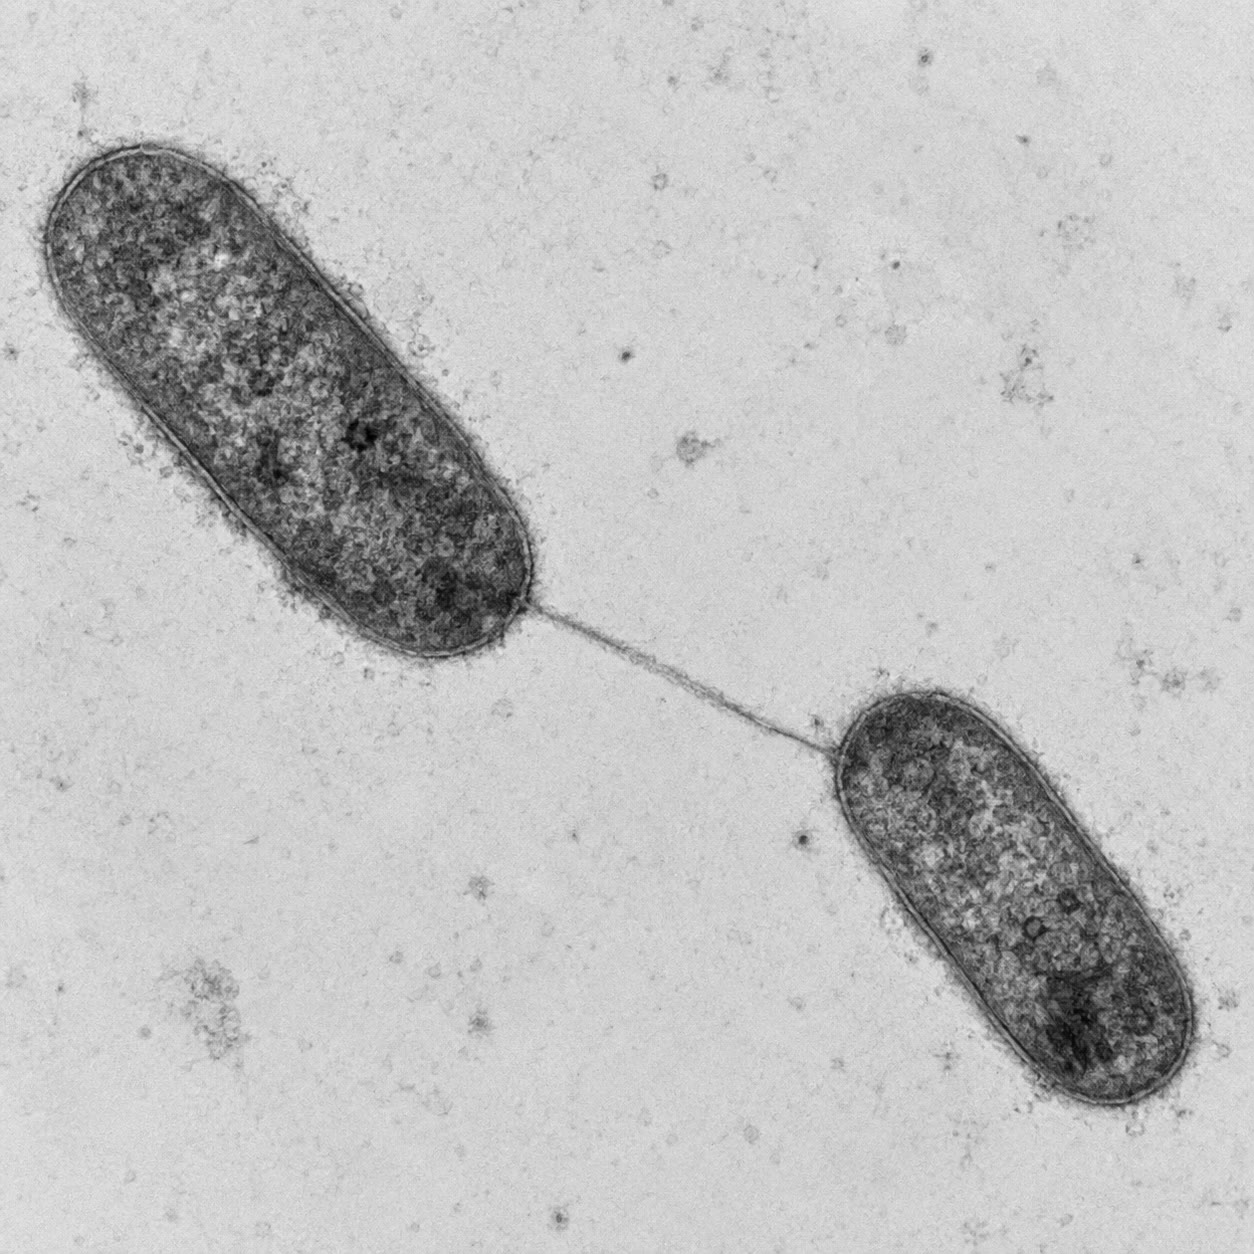
\includegraphics[width=0.42\linewidth]{images/book4/ai/b4-03-conjugation-tem.jpg}

{\small Dos bacterias unidas por un pilus conjugativo, vistas al
microscopio electrónico de transmisión: el puente por el que pasa el
\omterm{def:b2:unicellular-diversity:prokaryote}{plásmido}.}
\end{omfigure}

\begin{example}[La resistencia en movimiento]\label{ex:b2:genome-diversification:resistance}
Un gen de resistencia suele surgir una sola vez, por \omterm{def:b2:genome-diversification:mutation}{mutación} o a partir
de la bacteria del suelo que fabrica el antibiótico, y después viaja: de
un cromosoma a un \omterm{def:b2:genome-diversification:transposon}{transposón}, del \omterm{def:b2:genome-diversification:transposon}{transposón} a un \omterm{def:b2:unicellular-diversity:prokaryote}{plásmido} conjugativo,
del \omterm{def:b2:unicellular-diversity:prokaryote}{plásmido} a otras especies por conjugación y a otras cepas por
\omterm{def:b2:genome-diversification:hgt}{transducción}, y de vuelta a un cromosoma por \omterm{def:b2:genome-diversification:hgt}{transformación}. En Japón se
encontraron en los años cincuenta, pocos años después de que los
fármacos empezaran a usarse, \omterm{def:b2:unicellular-diversity:prokaryote}{plásmidos} portadores de cinco o seis
resistencias a la vez (reunidas en \emph{integrones}, que capturan
casetes génicos); el gen de la carbapenemasa NDM-1, detectado por primera
vez en 2008, llegó a todos los continentes en tres años a bordo de un
\omterm{def:b2:unicellular-diversity:prokaryote}{plásmido}. La evolución de la resistencia no es, en su mayor parte, la
evolución de genes nuevos, sino el desplazamiento de genes antiguos.
\end{example}

\section{Duplicación: genes y genomas}

\begin{proposition}[Duplicación génica y familias de genes]\label{prop:b2:genome-diversification:duplication}
\index{duplicación génica}\index{familia de genes}\index{entrecruzamiento desigual}
Cuando dos secuencias parecidas están en tándem en un cromosoma, los
homólogos pueden aparearse desalineados en la meiosis y entrecruzarse de
forma desigual, de modo que un producto lleva tres copias y el otro una.
Un gen duplicado es redundante: una copia puede mantener la función
antigua mientras la otra acumula \omterm{def:b2:genome-diversification:mutation}{mutaciones} libremente --- lo habitual es
que degenere en un \emph{pseudogén}; a veces adquiere una función nueva
(\emph{neofuncionalización}) o una parte de la antigua
(\emph{subfuncionalización}). Repetido a lo largo de cientos de millones
de años, esto construye \emph{\omterm{prop:b2:genome-diversification:duplication}{familias de genes}}: las globinas (un único
gen ancestral dio la mioglobina, el grupo $\alpha$ y el grupo
$\beta$, con miembros embrionarios, fetales y adultos que se expresan
por turnos), los receptores olfativos (mil genes en un ratón), los genes
homeobox, las cristalinas del cristalino. La mayoría de los genes de un
genoma pertenece a una familia, y la duplicación es la principal fuente
de genes nuevos.
\end{proposition}
\begin{proof}[Evidencia]
El grupo de la $\beta$-globina humana, en el cromosoma 11, contiene cinco
genes funcionales ($\varepsilon$, $^{G}\gamma$, $^{A}\gamma$,
$\delta$, $\beta$) y un pseudogén, en el orden en que se activan durante
el desarrollo, todos con la misma estructura de exones e intrones, y sus
secuencias son tanto más parecidas cuanto más recientemente divergieron;
el grupo $\alpha$, en el cromosoma 16, tiene la misma arquitectura. Las
deleciones de uno o más genes $\alpha$, producidas por \omterm{prop:b2:genome-diversification:duplication}{entrecruzamiento
desigual} entre las copias casi idénticas, son frecuentes y causan la
$\alpha$-talasemia; el producto recíproco, un cromosoma con tres genes
$\alpha$, se encuentra en las mismas poblaciones.
\end{proof}

\begin{omfigure}
\begin{tikzpicture}[every node/.style={font=\scriptsize}]
  % unequal crossing over
  \begin{scope}
    \draw[very thick, gray] (0,1.2) -- (5,1.2);
    \fill[omDef!70] (1.0,1.05) rectangle (2.0,1.35); \fill[omDef!70] (2.4,1.05) rectangle (3.4,1.35);
    \draw[very thick, gray] (0,0) -- (5,0);
    \fill[omDef!70] (1.0,-0.15) rectangle (2.0,0.15); \fill[omDef!70] (2.4,-0.15) rectangle (3.4,0.15);
    \node[above] at (1.5,1.35) {A}; \node[above] at (2.9,1.35) {A$'$};
    \draw[very thick, omThm] (2.9,1.05) -- (1.5,0.15);
    \node[align=center] at (2.5,-0.6) {los homólogos desalineados\\se entrecruzan de forma desigual};
    \draw[->, thick, gray] (5.3,0.6) -- (6.1,0.6);
    % products
    \draw[very thick, gray] (6.5,1.2) -- (11.5,1.2);
    \fill[omDef!70] (7.5,1.05) rectangle (8.5,1.35); \fill[omDef!70] (8.9,1.05) rectangle (9.9,1.35); \fill[omDef!70] (10.3,1.05) rectangle (11.3,1.35);
    \node[above] at (9.4,1.35) {tres copias};
    \draw[very thick, gray] (6.5,0) -- (11.5,0);
    \fill[omDef!70] (7.5,-0.15) rectangle (8.5,0.15);
    \node[above] at (8.0,0.15) {una copia};
  \end{scope}
  % globin family tree
  \begin{scope}[yshift=-3.6cm]
    \draw[thick] (2,2.2) -- (2,1.7);
    \draw[thick] (0.5,1.7) -- (3.5,1.7);
    \draw[thick] (0.5,1.7) -- (0.5,0.4); \node[below] at (0.5,0.4) {mioglobina};
    \draw[thick] (3.5,1.7) -- (3.5,1.2);
    \draw[thick] (2.3,1.2) -- (4.7,1.2);
    \draw[thick] (2.3,1.2) -- (2.3,0.4); \node[below] at (2.3,0.4) {familia $\alpha$};
    \draw[thick] (4.7,1.2) -- (4.7,0.9);
    \draw[thick] (3.6,0.9) -- (5.8,0.9);
    \draw[thick] (3.6,0.9) -- (3.6,0.4); \node[below] at (3.6,0.4) {$\varepsilon,\gamma$};
    \draw[thick] (5.8,0.9) -- (5.8,0.7);
    \draw[thick] (5.2,0.7) -- (6.4,0.7);
    \draw[thick] (5.2,0.7) -- (5.2,0.4); \node[below] at (5.2,0.4) {$\delta$};
    \draw[thick] (6.4,0.7) -- (6.4,0.4); \node[below] at (6.4,0.4) {$\beta$};
    \node[anchor=west, align=left] at (7.2,1.7) {duplicaciones de un gen ancestral de globina:\\antes de los vertebrados (mioglobina/hemoglobina),\\hace $\sim$450 millones de años ($\alpha$/$\beta$),\\y después dentro del grupo $\beta$ (embrionaria, fetal, adulta)};
    \node[anchor=east, gray] at (1.9,2.1) {globina ancestral};
  \end{scope}
\end{tikzpicture}

{\small Arriba: el \omterm{prop:b2:genome-diversification:duplication}{entrecruzamiento desigual} entre copias en tándem
desalineadas produce un cromosoma con tres copias y otro con una sola.
Abajo: la familia de las globinas, construida por duplicaciones y
divergencias sucesivas.}
\end{omfigure}

\begin{definition}[Poliploidía]\label{def:b2:genome-diversification:polyploidy}
\index{poliploidía}\index{alopoliploide}\index{autopoliploide}
Un \emph{poliploide} lleva más de dos juegos cromosómicos completos. Un
\emph{autopoliploide} tiene varios juegos de una misma especie (una
meiosis fallida da un gameto diploide; dos de esos gametos dan un
tetraploide); un \emph{alopoliploide} combina los juegos de dos especies
tras una hibridación. El híbrido diploide AB, sin homólogo para ningún
cromosoma, no puede aparearlos en la meiosis y es estéril; si su genoma
se duplica a AABB, cada cromosoma vuelve a tener pareja, la meiosis
funciona y la nueva planta es fértil --- pero no puede cruzarse con
ninguno de sus progenitores (un descendiente AAB es estéril). La
poliploidía crea así una especie nueva en un solo paso, y alrededor de un
tercio de las especies de plantas con flores surgieron de esta manera: el
trigo harinero es un hexaploide AABBDD de tres gramíneas, la fresa de
jardín un octoploide, el algodón y el tabaco alotetraploides, y el propio
linaje de los vertebrados duplicó su genoma dos veces cerca de su origen.
Los poliploides suelen ser más grandes que sus antepasados diploides (más
ADN, células mayores) y muy apreciados por los mejoradores.
\end{definition}

\begin{omfigure}
\begin{tikzpicture}[every node/.style={font=\scriptsize}]
  \node[draw, rounded corners, fill=omDef!10, align=center] (a) at (0,0) {\emph{T.~urartu}\\AA, $2n = 14$};
  \node[draw, rounded corners, fill=omDef!10, align=center] (b) at (3.4,0) {\emph{Aegilops}\\BB, $2n = 14$};
  \node[draw, rounded corners, fill=omProp!15, align=center] (ab) at (1.7,-1.5) {híbrido AB\\$n = 14$, estéril};
  \node[draw, rounded corners, fill=omExo!25, align=center] (aabb) at (1.7,-3.1) {trigo almidonero AABB\\$2n = 28$, fértil};
  \node[draw, rounded corners, fill=omDef!10, align=center] (d) at (6.4,-3.1) {\emph{Ae.~tauschii}\\DD, $2n = 14$};
  \node[draw, rounded corners, fill=omProp!15, align=center] (abd) at (4.0,-4.6) {híbrido ABD\\$3n = 21$, estéril};
  \node[draw, rounded corners, fill=omExo!25, align=center] (abd2) at (4.0,-6.1) {trigo harinero AABBDD\\$2n = 42$, fértil};
  \draw[->, thick] (a) -- (ab); \draw[->, thick] (b) -- (ab);
  \draw[->, thick] (ab) -- (aabb) node[midway, right] {duplicación del genoma};
  \draw[->, thick] (aabb) -- (abd); \draw[->, thick] (d) -- (abd);
  \draw[->, thick] (abd) -- (abd2) node[midway, right] {duplicación del genoma};
  \node[anchor=west, align=left, gray] at (7.8,-1.5) {cada hibridación da una planta\\estéril con cromosomas sin pareja;\\cada duplicación restablece el\\apareamiento y la fertilidad --- y crea\\una especie que no puede retrocruzarse};
\end{tikzpicture}

{\small El origen del trigo harinero: dos hibridaciones, cada una seguida
de una duplicación del genoma, construyeron un hexaploide a partir de
tres gramíneas diploides en unos diez mil años.}
\end{omfigure}

\begin{omfigure}
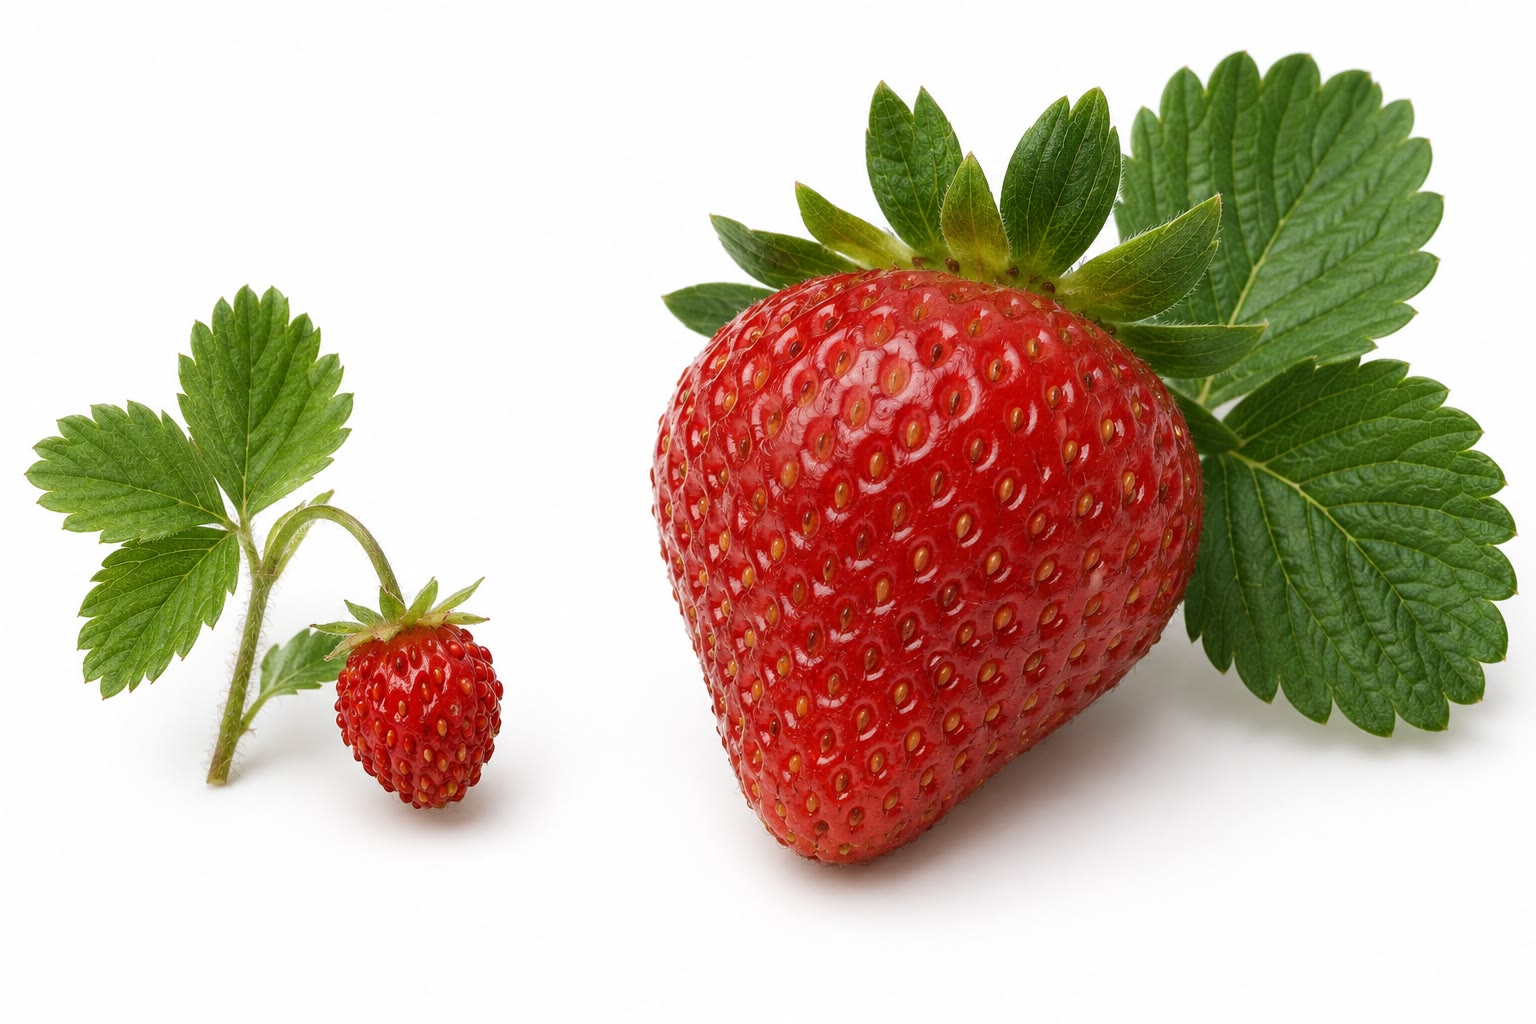
\includegraphics[width=0.55\linewidth]{images/book4/ai/b4-03-polyploid-strawberries.jpg}

{\small Una fresa silvestre diploide y la octoploide cultivada: el
\omterm{def:b2:genome-diversification:polyploidy}{poliploide}, con cuatro veces más ADN en cada célula, es la planta más
grande y la de fruto más grande.}
\end{omfigure}

\section{Azar y tasa}

\begin{proposition}[La mutación es aleatoria respecto a la necesidad]\label{prop:b2:genome-diversification:random}
\index{mutación!carácter aleatorio de la}
El \omterm{thm:b2:genome-diversification:luria}{test de fluctuación} y la siembra en réplica muestran que una \omterm{def:b2:genome-diversification:mutation}{mutación}
útil en un ambiente nuevo surge con la misma frecuencia esté o no
presente ese ambiente: el ambiente selecciona entre las \omterm{def:b2:genome-diversification:mutation}{mutaciones}, no
las provoca. La \omterm{def:b2:genome-diversification:mutation}{mutación} no es aleatoria en todos los sentidos --- las
transiciones superan en número a las transversiones, los dinucleótidos
CpG mutan diez veces más deprisa que otros sitios (su citosina metilada
se desamina a timina, que la reparación no reconoce como extraña),
algunas regiones son puntos calientes y el estrés puede elevar la tasa
global ---, pero es ciega a las consecuencias. La propia \omterm{thm:b2:genome-diversification:rate}{tasa de
mutación} es un rasgo heredable, y la selección la ajusta: demasiado alta,
y cada generación hereda cambios perjudiciales; demasiado baja, y la
población no puede seguir a un mundo cambiante. Las cepas mutadoras
ganan brevemente en un hospital y pierden a la larga, y la tasa de
$10^{-9}$ por base en la que se sitúan la mayoría de las células es un
compromiso entre el coste de los errores y el coste de la corrección.
\end{proposition}

\section{Ejercicios}

\begin{exercise}[$\star$]\label{exo:b2:genome-diversification:1}
Clasifíquese cada cambio del codón GAA (glutamato): GAG; GTA; TAA;
inserción de una C tras la primera base. ¿Cuál es una transición y cuál
una transversión?
\end{exercise}

\begin{exercise}[$\star$]\label{exo:b2:genome-diversification:2}
Con $u = \qty{5e-10}{}$ por par de bases y por replicación y $G =
\qty{4.6e6}{}$, ¿cuántas \omterm{def:b2:genome-diversification:mutation}{mutaciones} nuevas produce en promedio una
división de \emph{E.~coli}? ¿Cuántas por generación en un cultivo de
$10^{9}$ células?
\end{exercise}

\begin{exercise}[$\star$]\label{exo:b2:genome-diversification:3}
Nómbrense las tres vías de \omterm{def:b2:genome-diversification:hgt}{transferencia horizontal de genes} y dígase,
para cada una, qué requiere (contacto, un virus, ADN libre) y qué suele
transferir.
\end{exercise}

\begin{exercise}[$\star$]\label{exo:b2:genome-diversification:4}
Distíngase la autopoliploidía de la alopoliploidía, con un ejemplo de
cada una, y explíquese por qué un híbrido diploide de dos especies suele
ser estéril.
\end{exercise}

\begin{exercise}[$\star\star$]\label{exo:b2:genome-diversification:5}
Una línea germinal humana acumula $u = \qty{1.2e-8}{}$ \omterm{def:b2:genome-diversification:mutation}{mutaciones} por
par de bases y por generación en un genoma haploide de \qty{3.2e9}{} pares
de bases. ¿Cuántas \omterm{def:b2:genome-diversification:mutation}{mutaciones} nuevas lleva un hijo? Si el \qty{1.5}{\%}
del genoma codifica proteínas y el \qty{70}{\%} de las sustituciones
codificantes cambia un aminoácido, ¿cuántos cambios de aminoácido nuevos
lleva el hijo?
\end{exercise}

\begin{exercise}[$\star\star$]\label{exo:b2:genome-diversification:6}
Un cultivo crece de $10^{3}$ a $10^{9}$ células; una \omterm{def:b2:genome-diversification:mutation}{mutación} dada
ocurre con $m = \qty{2e-8}{}$ por división. Calcúlense el número esperado
de sucesos de \omterm{def:b2:genome-diversification:mutation}{mutación} y el de células mutantes. ¿Por qué la fracción de
cultivos sin mutante no sirve aquí para medir $m$, y qué tamaño de
cultivo la haría útil?
\end{exercise}

\begin{exercise}[$\star\star$]\label{exo:b2:genome-diversification:7}
La citosina se desamina a uracilo; la 5-metilcitosina se desamina a
timina. Explíquese por qué la primera lesión se repara eficazmente y la
segunda no, y dedúzcase por qué los sitios CpG (donde la citosina está
metilada) son puntos calientes de \omterm{def:b2:genome-diversification:mutation}{mutación} y más escasos en el genoma de
lo que predeciría el azar.
\end{exercise}

\begin{exercise}[$\star\star$]\label{exo:b2:genome-diversification:8}
En un experimento de apareamiento interrumpido, cuatro genes entran en el
receptor a los 8, 17, 25 y \qty{40}{min}; el cromosoma entero
(\qty{4.6}{Mb}) tardaría \qty{100}{min}. Conviértanse los tiempos en
posiciones en kilobases y calcúlense las distancias entre genes
consecutivos.
\end{exercise}

\begin{exercise}[$\star\star$]\label{exo:b2:genome-diversification:9}
Dibújense el apareamiento y el entrecruzamiento que convierten dos
cromosomas con dos genes de $\alpha$-globina en tándem cada uno en uno con
tres y otro con uno. Una persona hereda un cromosoma de un solo gen de
cada progenitor: ¿cuántos genes $\alpha$ tiene, y qué cabe esperar de su
hemoglobina?
\end{exercise}

\begin{exercise}[$\star\star\star$]\label{exo:b2:genome-diversification:10}
El trigo harinero es AABBDD, con $2n = 42$. Dese el número de cromosomas
de sus gametos, de los híbridos estériles de cada etapa de su origen y de
un cruzamiento entre el trigo harinero y el almidonero (AABB). Explíquese
en términos de apareamiento meiótico por qué cada duplicación restableció
la fertilidad y por qué el hexaploide no puede retrocruzarse con sus
progenitores.
\end{exercise}

\begin{exercise}[$\star\star\star$]\label{exo:b2:genome-diversification:11}
En una población intestinal de $N = 10^{9}$ bacterias, un \omterm{def:b2:unicellular-diversity:prokaryote}{plásmido} de
resistencia se propaga por conjugación a un ritmo proporcional a los
encuentros entre portadoras $R$ y no portadoras $N - R$: $\mathrm{d}R/\mathrm{d}t =
\gamma R (N - R)$ con $\gamma N = \qty{0.5}{h^{-1}}$. Resuélvase partiendo
de una portadora y calcúlese el tiempo necesario para que la mitad de la
población lleve el \omterm{def:b2:unicellular-diversity:prokaryote}{plásmido}. ¿Qué ocurre si después se retira el
antibiótico y el \omterm{def:b2:unicellular-diversity:prokaryote}{plásmido} le cuesta a su hospedador un \qty{5}{\%} de tasa
de crecimiento?
\end{exercise}

\begin{exercise}[$\star\star\star$]\label{exo:b2:genome-diversification:12}
``La \omterm{def:b2:genome-diversification:mutation}{mutación} es aleatoria; la evolución no.'' Discútase a partir del
\omterm{thm:b2:genome-diversification:luria}{test de fluctuación}, de la siembra en réplica y del hecho de que la propia
\omterm{thm:b2:genome-diversification:rate}{tasa de mutación} está sometida a selección.
\end{exercise}

\section{Problema: un test de fluctuación}

\begin{problem}[{Problema de fin de semana --- se realiza y analiza un
test de fluctuación, se extrae de él la tasa de mutación de una cepa y se
lleva a la escala de su genoma y de su población, se modeliza la
propagación de un plásmido de resistencia y se sopesa el coste de un
mutador, hasta llegar a la tasa de mutación por base de la cepa y al
tiempo que tarda el plásmido en imponerse}]
\label{pb:b2:genome-diversification:1}
Se inician veinte cultivos de \emph{E.~coli}, cada uno a partir de
\num{100} células en \qty{0.2}{mL}, y se dejan crecer hasta $N = \qty{2e8}{}$
células; cada uno se siembra después en una placa con un bacteriófago y
se cuentan las colonias resistentes: 0, 0, 0, 1, 0, 0, 3, 0, 0, 1, 0, 0,
0, 0, 107, 0, 2, 0, 0, 5. En paralelo, se toman veinte muestras de
\qty{0.2}{mL} de un único cultivo grande de la misma densidad y se
siembran igual: 14, 15, 13, 21, 15, 14, 26, 16, 20, 13, 17, 12, 18, 14,
16, 19, 15, 13, 17, 16. Genoma: \qty{4.6e6}{} pares de bases, el
\qty{88}{\%} codificante. La resistencia al fago puede surgir por
cualquiera de \num{20} cambios distintos de una sola base en un gen de
receptor.

\medskip
\noindent\textbf{Parte I --- El test.}
\begin{enumerate}
  \item Calcúlense la media y la varianza de los veinte cultivos
        independientes.
  \item Calcúlense la media y la varianza de las veinte muestras.
  \item En una distribución de Poisson la varianza es igual a la media.
        ¿Qué serie es de Poisson, y qué dice la distribución de cada serie
        sobre \emph{cuándo} ocurrieron las \omterm{def:b2:genome-diversification:mutation}{mutaciones}?
  \item Explíquese el recuento de 107.
  \item ¿Cuántos cultivos independientes no contienen ningún mutante?
        Úsese $p_0 = e^{-m(N - N_0)}$ para estimar $m$, la \omterm{thm:b2:genome-diversification:rate}{tasa de
        mutación} a la resistencia por división celular.
  \item Calcúlese el número esperado de células mutantes por cultivo a
        partir de $mN\ln(N/N_0)$ y compárese con la media observada.
  \item ¿Por qué las muestras del cultivo único no habrían servido para
        estimar $m$ por el método de $p_0$?
\end{enumerate}

\medskip
\noindent\textbf{Parte II --- A escala del genoma.}
\begin{enumerate}[resume]
  \item Dedúzcase la \omterm{thm:b2:genome-diversification:rate}{tasa de mutación} $u$ por par de bases y por
        replicación a partir de $m$ y del número de cambios que confieren
        resistencia.
  \item Calcúlese el número medio de \omterm{def:b2:genome-diversification:mutation}{mutaciones} nuevas por genoma y por
        replicación, $U$.
  \item Un cultivo de un litro a $10^{9}$ células por mililitro se duplica
        una vez. ¿Cuántas \omterm{def:b2:genome-diversification:mutation}{mutaciones} nuevas surgen en la población?
  \item ¿Cuántos cambios distintos de una sola base son posibles en este
        genoma? En promedio, ¿cuántas veces surge cada uno en esa única
        duplicación?
  \item Explíquese por qué, en una población así, la resistencia a
        cualquier antibiótico que una sola \omterm{def:b2:genome-diversification:mutation}{mutación} puede vencer está
        prácticamente garantizada.
  \item Explíquese, con una cifra, por qué combinar dos antibióticos que
        requieren dos \omterm{def:b2:genome-diversification:mutation}{mutaciones} independientes cambia la situación.
\end{enumerate}

\medskip
\noindent\textbf{Parte III --- Un \omterm{def:b2:unicellular-diversity:prokaryote}{plásmido} se propaga.}
En un intestino con $N = 10^{9}$ células, una célula adquiere un \omterm{def:b2:unicellular-diversity:prokaryote}{plásmido}
conjugativo de resistencia. Las portadoras $R$ lo transmiten por contacto:
$\mathrm{d}R/\mathrm{d}t = \gamma R(N - R)$, con $\gamma N =
\qty{0.5}{h^{-1}}$.
\begin{enumerate}[resume]
  \item Demuéstrese que $R(t) = N/\bigl(1 + (N - 1)e^{-\gamma N t}\bigr)$
        es solución de la ecuación con $R(0) = 1$.
  \item Calcúlese el momento en que la mitad de las células lleva el
        \omterm{def:b2:unicellular-diversity:prokaryote}{plásmido}.
  \item Calcúlese el momento en que lo lleva el \qty{99}{\%}.
  \item ¿Cuántos sucesos de conjugación por hora tienen lugar en el
        momento en que la mitad de las células son portadoras?
  \item Compárese con el tiempo que tarda un \emph{mutante} resistente en
        alcanzar la mitad de la población creciendo un \qty{10}{\%} más
        deprisa que el resto bajo el antibiótico (\omterm{def:b2:unicellular-diversity:division}{tiempo de generación} de
        \qty{1}{h} para las células sensibles): partiendo de una célula,
        ¿cuánto tarda?
  \item Conclúyase por qué la resistencia se propaga sobre todo por
        transferencia y no por descendencia.
\end{enumerate}

\medskip
\noindent\textbf{Parte IV --- Un mutador.}
Una cepa sin reparación de desapareamientos muta \num{100} veces más
deprisa. Supóngase que el \qty{30}{\%} de las \omterm{def:b2:genome-diversification:mutation}{mutaciones} en secuencia
codificante son perjudiciales.
\begin{enumerate}[resume]
  \item Calcúlense su $U$ y el número medio de \omterm{def:b2:genome-diversification:mutation}{mutaciones} perjudiciales
        por célula y por generación.
  \item Al cabo de \num{200} generaciones, ¿qué fracción de los
        descendientes de un linaje no lleva ninguna \omterm{def:b2:genome-diversification:mutation}{mutación} perjudicial
        (Poisson)?
  \item Calcúlese lo mismo para el tipo silvestre.
  \item En el \omterm{thm:b2:genome-diversification:luria}{test de fluctuación} anterior, ¿qué recuento medio habría
        dado el mutador, y qué fracción de cultivos sin mutante?
  \item Explíquese en dos frases por qué se encuentran mutadores entre los
        aislados hospitalarios y por qué son raros en la naturaleza.
  \item Enúnciese el resultado: $m$, $u$ y $U$ para la cepa, y los tiempos
        que tarda el \omterm{def:b2:unicellular-diversity:prokaryote}{plásmido} en alcanzar la mitad y el \qty{99}{\%} del
        intestino.
\end{enumerate}
\end{problem}
